\section{Betriebs-, Infrastruktur- und Ausbildungskosten}
\label{s:Kosten}
In diesem Unterkapitel werden die Kostenstrukturen vorgestellt, 
wobei bei Betriebskosten auf die Kosten der Fluggesellschaft
eingegangen wird und bei der Infrastruktur, aufgrund der dazugehörigen Kapitalkosten, auf die Flughäfen.
%
\subsection{Betriebskosten einer Fluggesellschaft}

Die Betriebskosten einer Flugzeugabfertigung werden auf Direct Operating Costs ($DOC$) und Indirect Operating Costs 
($IOC$) aufgeteilt, welche auch Einzel- und\\ Gemeinkosten genannt werden \cite{conrady2019luftverkehr}. 
Nach Mensen \cite{mensen2013handbuch} können $DOC$ einem bestimmten Flugzeug oder einer Strecke zugeordnet 
werden und normalerweise als DOC pro Flugstunde, pro Kilometer, pro Passagierkilometer oder pro Blockstunde 
berechnet werden. IOC werden nicht direkt einem Flug zugewiesen, sondern fallen für den gesamten Betrieb an, 
z.B. für zeitabhängige Instandhaltungs-, Verwaltungs- und Infrastrukturkosten. 
Nach der Beschäftigungsabhängigkeit werden die Kosten auf fixe und variable Kosten aufgeteilt. 
Fixe Kosten stehen unabhängig zu dem Betrieb (z.B. Kapitalkosten, Versicherung, Personalkosten), 
die variablen Kosten hingegen ändern sich Bezug auf die Beschäftigung.
%
Die Kostenstruktur einer Fluggesellschaft kann mit der Abbildung \ref{doc} veranschaulicht werden.
%
\begin{figure}[h]
	\centering
	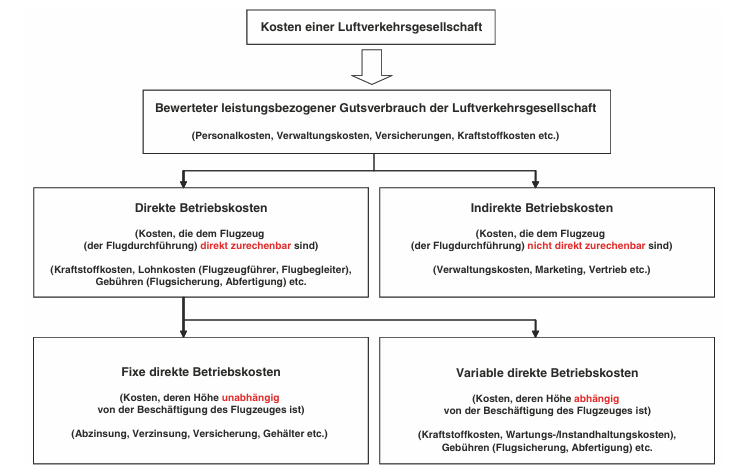
\includegraphics[width=0.9\linewidth]{Bilder/Systematik der DOC_Berechnung.png}
	\caption[Kostenstruktur einer Fluggesellschaft]{Kostenstruktur einer Fluggesellschaft \cite{mensen2013handbuch}}
	\label{doc}
\end{figure}

Betriebskosten sind von dem Flugzeugtyp abhängig, deswegen ist es für den Betreiber 
wichtig vor der Anschaffung zu untersuchen, 
ob ein Flugzeug mit einem alternativen Antrieb rentabel ist. 
Die neuen Regularien der \ce{CO2}-Reduktion können einen Anreiz oder sogar 
eine Verpflichtung für die Fluggesellschaften schaffen, um eine bestmögliche Lösung für eine Flotte zu finden. 
Weitere Aspekte politischer Anreize werden im folgenden Unterkapitel \ref{s:Klimapolitische Maßnahmen} betrachtet.
%
Es gibt verschiedene bereits vorgestellte Formeln für die Berechnung der DOC \cite{scholz_design_evaluation_doc}. 
Die meisten davon schließen die gleichen Kostenfaktoren ein, 
unterscheiden sich jedoch in der Rechnungsweise für einzelne Kosten.
Einberechnet werden Treibstoffkosten, Crewkosten, Wartungskosten, kapitalbezogene Kosten, sowie Entgelte und Gebühren.\\

%
\textbf{Treibstoffkosten} sind ein erheblicher Teil der Betriebskosten. 
In den USA sind ein Drittel aller Gesamtkosten (TOC) aller Fluggesellschaften 
die Kosten für Treibstoff und Öl, in Korrelation dazu beträgt 
die Abfertigung am Flughafen ein Sechstel \cite{conrady2019luftverkehr}. 
Im Jahr 2023 wurden etwa 92 Milliarden Gallonen Kraftstoff durch der 
Luftfahrtindustrie verbraucht und somit betrug die Treibstoffrechnung fast 32 \% 
aller Betriebskosten der Luftfahrt \cite{iata_industry_statistics_2024}.
Die jährlichen Steigerungen der Preise für fossile Rohstoffe können die nachhaltige Initiative fördern. \\
%Kesorinpreis im Jahr 2022 betrug USD 136/bbl, prognostiziert wird jedoch ...
%
%"Betrachtet man den aktuellen Stand der kommerziellen Luftfahrt, so macht fossiles ATF den 
%größten Teil des Energieverbrauchs im Luftverkehr aus, wobei Jet A und Jet A-1 überwiegend verwendet werden" %wo kommt das her?
%
%Technikkosten (Wartung, Reparatur, Instandhaltung MRO) - 
%es gibt unterschiedliche Typen von Wartung, die Kontrolle was am Vorfeld bei einem 
%Turnaround passiert ist die line maintenance (prüfung von Reifendruck und Ölständen), Flughafenentgelte und Handlingkosten: 
%Bodenabfertigung besteht aus Passagierabfertigung, Fracht-, Gepäckabfertigung und VorfelddiensteFlugzeugabfertigung ist direkte Kosten, 
%Passagierkosten indirekte Kosten, Kapital- und Abschreibungskosten \cite{conrady2019luftverkehr}. 
%Conrady bescheibt die Cockpit Crew als auch Cabin Crew, so Gehälter, Reisekosten, Schulungskosten. Es gibt jedoch nur wenige Arbeiten, 
%die die Ausbildungskosten erwähnen. Auch Handling Agents Kosten gibt es nicht viel Information zu finden. Es kann damit zurückgeführt werden, dass
%sind unabhängige von Fluggesellschaften Handling Agents für Abfertigung zuständig und nicht die Fluggesellschaften Kosten dafür übernehmen.
%
\textbf{Crewkosten} sind auch ein Bestandteil der direkten Betriebskosten. 
Zu einer Crew gehören Piloten und Kabinen-Besatzung.
Nach Conrady \cite{conrady2019luftverkehr} bestehen die Besatzungs-\\kosten aus 
Gehältern, Reise- und Schulungskosten. Es gibt jedoch nur wenige Quellen, 
die bei der Berechnung der Betriebskosten die Ausbildungskosten erwähnen. \\
%
\textbf{Wartungskosten} eines Flugzeugs fassen die Arbeitskosten für Beschäftigte
und benötigten Materialien für die Wartung zusammen.
Außerdem werden die Kosten in Wartung der Zelle und den Triebwerken unterteilt \cite{wang2021research}. 
Meistens werden diese Komponenten von unterschiedlichen Unternehmen hergestellt (Quelle).%%%%%%%%%%%%%%%%%%%%%%%%% oder Satz weg?
Am Vorfeld bei der Luftfahrzeugabfertigung findet eine \textit{Line Maintenance} statt, 
dabei wird der Reifendruck und Ölstände überprüft \cite{conrady2019luftverkehr}. 
Darüber hinaus finden eine Reihe anderer regelmäßiger Kontrollen statt.
Wartungskosten hängen von Auslastung eines Flugzeugs ab, je mehr sich ein Flugzeug in Betrieb befindet, desto höhere 
Kosten sind zu erwarten. %schnellere Wartung man braucht, desto teurere Komponente man braucht.
%Wartungskosten wachsen mit der Größe des Flugzeugs, da mehr Personal oder mehr Zeit für die Wartung benötigt ist.
%
%Die Kurzstrecken-Flugzeuge sind mehr mit größerer Anzahl an Landungsgebühren und größere Treibstoffverbrauch verbunden sind, da 
%der Start und die Landung sind die Treibstoff aufwendigste Prozesse im ganzen Flug.
%
Je nach Flotte sind Ersparnisse möglich, wenn die Fluggesellschaften mehrere Flugzeuge vom gleichen Typ anschaffen \cite{conrady2019luftverkehr}. 
In diesem Fall sind weniger Schulungen für Techniker notwendig.\\
%
%
%Eine Reihe anderen Kosten, die für die Arbeit vielleicht nicht relevant?: Flugsicherungsgebühren, Versicherungskosten (bleiben), 
%Servicekosten, Marketing- und Vertriebskosten, Kpsten der allgemeinen Verwaltung, 
%Diese werden aufgrund der Komplexität der Berechnungen und der begrenzten Verfügbarkeit von Daten nicht weiter betrachtet.
%
%
%Preis für Treibstoffversorgung für kurzfristige Perioden kann folgend berechnet werden \cite{iata_saf_procurement_2024}: nicht sicher, ob die Formel nehme
%PRA-Bewertung (Risikobewertung??? Durchschnitt der Vorperiode) + Logistikkosten + zusätzliche Gebühren + Lieferantenmarge
%
Unter \textbf{kapitalbezogenen Kosten} versteht man Kosten, die vom Flugzeuganschaffungspreis abhängig sind.
Darunter sind Abschreibung, Verzinsung und Versicherung zu verzeichnen.
Abschreibungskosten sind ein Teil der Kapitalkosten für das Flugzeug, 
die auf einen festgelegten Zeitraum, in welchem Flugzeug genutzt wird, verteilt werden \cite{conrady2019luftverkehr}.
Abschreibungswerte unterscheiden sich je nach Fluggesellschaft.
Die Abschreibungskosten können auch auf die Infrastruktur bezogen werden. 
Flugzeuge werden gegen Rumpfschäden oder andere Arten von Schäden versichert \cite{scholz_design_evaluation_doc}.  \\
%
%Conceptual_Design_and_Operating_Costs_Evaluation_of_a_19-seat_All-Electric_Aircraft_for_Regional_Aviation
%"die Zins- und Abschreibungskosten sinken tendenziell bei hoher Tagesauslastung"
%20 Prozent in Motorwartung verringert DOC um 4%
%
%
%Arten Wartung: DMC are the maintenance costs caused directly by the aircraft; 
%Wartung "line maintenance cost; periodic maintenance cost; workshop direct maintenance cost; and overhaul cost."
In dieser Arbeit wird der Fokus auf die direkten Betriebskosten gelegt und die indirekten Betriebskosten, wie Kosten für 
allgemeine Verwaltung, Marketing- und Servicekosten, werden wegen geringerer Relevanz nicht betrachtet.\\
%
\subsection{Infrastrukturkosten}
%
Durch den Anstieg der Nachfrage nach innovativen Antrieben sind Änderungen an der Flughafeninfrastruktur notwendig.
%
Die Infrastruktur eines Flughafens gibt vor, über welche Kapazitäten einen Flughafen verfügt.
Die Infrastrukturkosten eines Flughafens bestehen aus Kosten für luft- und landseitige Anlagen \cite{fur2003infrastrukturkosten}. 
Landseitige sind die Einrichtungen die zum Flughafen gehören wie bspw. Terminal oder administrative Gebäude. 
Zur luftseitigen Infrastruktur gehören Start-/Landebahn, Rollbahn, Vorfeld, Flugsicherheitsinfrastruktur und -ausrüstung. 
Die Infrastruktur kann unterschiedlich finanziert werden.
Flughafengebühren, wie Lande-, \\Lärm-, Emissions-, Abstell-, Passagier- und Frachtgebühr 
tragen zur Finanzierung des Flughafens bei.

Infrastrukturkosten setzen sich nicht nur aus Anschaffungs-/Investitionskosten (Kapitalanforderungen), 
sondern auch durch Kosten für die Instandhaltung der Anlagen und Betriebskosten zusammen.
Kapitalkosten (wie Verzinsung und Abschreibung), die mit Infrastrukturinvestitionen zusammenhängen 
machen einen großen Teil der Gesamtkosten eines Flughafens aus \cite{wittmer2011aviation}.
%"Infrastrukturträger im Luftverkehr sind neben den Flughäfen die 
%Bodenabfertigungsdienste, Kommunikationseinrichtungen (z. B. SITA) und Flugsicherungseinrichtungen 
%(Radar-, Funknavigationsanlagen, Flugverkehrskontrolle ATC = Air traffic control)."  %file:///C:/Users/henri/Downloads/Lufrverkehr_10.1524_9783486841848.pdf
%
Flughäfen müssen wirtschaftliche Analysen nutzen, um Entscheidungen über Flughafeninvestitionen treffen zu können. %Bei Flughäfen mit beschränkten Bauschutzbereich muss für Erweiterung
Investitionsbeihilfen werden durch die Passagieranzahl des Flughafens bestimmt. 
Mit mehr als fünf Millionen Passagieren müssen Flughäfen ihre Kapitalkosten selbst tragen können \cite{conrady2019luftverkehr}. 
%"Allein  die Planfeststellungs-  und  Genehmigungsverfahren  für große  Infrastrukturprojekte dauern in  
%Deutschland im Durchschnitt 10  bis 15 Jahre."%https://www.researchgate.net/publication/279512505_Handlungsbedarf_fur_Planung_und_Nutzung_der_Flughafeninfrastruktur_in_Deutschland_Needs_for_Action_in_Planning_and_Use_of_Airport_Infrastructure_in_Germany
%
Über landseitige Anlagen finanzieren sich Flughäfen durch Mieten, Konzessionen und weitere Quellen \cite{fur2003infrastrukturkosten}.
Hat ein Flughafen regionale Bedeutung werden auch anderen Interessentengruppen an der Entwicklung teilnehmen.
Die Planung der Infrastrukturerweiterung oder -neubau muss in enger Zusammenarbeit 
zwischen den Stakeholdern (z.B. Regulierungsbehörden, Mitarbeitern, Anteilseignern, Kreditoren) stattfinden \cite{wittmer2011aviation}.
%
Außerdem müssen Infrastrukturentscheidungen mit den Interessen der Gesellschaft übereinstimmen \cite{WissenschaftlicherBeirat2011}. 

Diese Arbeit wird sich auf die Anschaffungskosten für neue Infrastruktur fokussieren und nicht mit 
laufenden Kosten, wie Betriebs-, Unterhalts- und Administrationskosten der Flughäfen arbeiten, 
da sie untergeordnete Relevanz haben.

\subsection{Ausbildungskosten}

Schulungen sind ein wichtiger Teil der Ausbildung. 
%Über was geht in der annex
Nach ICAO Annex 6 muss das Schulungsprogramm eine Kompetenzschulung für alle installierten Geräte umfassen.
Aufgrund zu erwartender neuer Antriebe werden ebenfalls neue Infrastruktur und Geräte benötigt, 
wodurch neue Gefahren im Luftverkehr entstehen können. % MAX: hier stimmt was nicht
Die erforderlichen Kenntnisse variieren je nach Einsatzbereich.
%
Wegen unzureichender Datenlage in dem Bereich ist schwierig die 
Ausbildungsdauer und damit verbundene Kosten präzise zu berechnen.
Aus diesem Grund wird auf eine detaillierte Analyse der Ausbildungskosten verzichtet 
und nur auf allgemein erforderliche Kenntnisse bei der Schulung hinweisen.
Dabei wird in dem Teil \ref{s:Neuartige Antriebe} auf die Sicherheitsaspekte und Gefahren 
beim Umgang mit den Antriebsarten eingegangen und %im Teil \ref{s:Änderungen durch neue Antriebe, Annahmen und Methodik}
die Schlussfolgerung für Ausbildungen zusammengefasst. %unsicher
%Wasserstoff: benötigt zusätzliche Fortbildung % MAX: das noch formulieren?

%Für Wasserstoff: 
%The goals of this training course include:
%• Familiarization with hydrogen safety properties.
%• To identify, evaluate, and address hydrogen system hazards.
%• To teach safe practices for design, materials selection, and hydrogen system operation.
%• physical principles and empirical observations on which these safe practices are based:
%• how to respond to emergency situations involving hydrogen
%• how to visualize safety concepts
%• identify numerous parameters important to hydrogen safety.

